Preprocessing is a fundamental step especially in this problem's context, as handwritten text tends to manifest chaotic nuances, at least for a computer. One could find it crucial to learn about the characteristics of cursive text in order to normalize a good deal of the redundant features. Some guidance zones when inspecting a line of text are shown in figure \ref{FigLineZones}. Two immaginary lines, namely the upperline (top) and the baseline (bottom), border the area (core region) that contains the major portion of the lowercase characters. The letters whose glyphs exceed that zone can situate themselves either into an upper area (ascenders region), like "b","h","l", or into the bottom area (descenders region), such as letters "g", "y", "q" \cite{Juan}.

\begin{figure}[htbp]
    \centering
        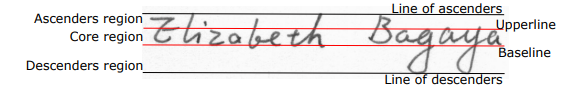
\includegraphics[scale=0.7]{figures/calligraphy_components}
    \caption{Calligraphy topological features \cite{Juan}}
    \label{FigLineZones}        
\end{figure}

A deviation in the angle of the baseline relative to the horizontal axis produces a slope \cite{Juan}. Correcting the slope may pose a great challenges as it may vary along the same line of text (imagine a line written in a style that starts parallel to the horizontal line and gradually curves itself down near the end of the page). In addition, writers tend to skew the letters vertically to the right (\ref{FigSlopeSlant}), therefore introducing a slant \cite{Juan}. 

\begin{figure}[htbp]
    \centering
        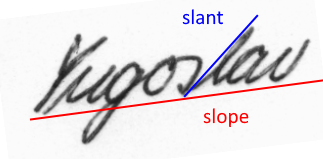
\includegraphics[scale=0.7]{figures/slope_slant.png}
    \caption{Slope and slant illustrated on an IAM sample}
    \label{FigSlopeSlant}        
\end{figure}

One slope and slant correction approach would be to identify the inclination angles and perform the corresponding geometric transformations to remove the irregularities. A noise removal would be preffered before manipulating the data \cite{Juan}.

Text segmentation refers to the process of finding the areas in a picture that contain textual data. The literature pick for this kind of task is some kind of convolutional deep learning model, such as the line counter algorithm \cite{linecounter}. One of the greatest challenge in line segmentation would be overlapping lines, which may happen when the line of ascenders intersects the line of descenders of the above text line \cite{Juan}. This is a fairly common occurence in lineated notebook scans.